\subsubsection{ Nguyên lý hoạt động}
Tác vụ "Temperature-Driven LED Blinking" được thiết kế nhằm điều khiển trạng thái chớp tắt của đèn cảnh báo LED1 thông qua dữ liệu nhiệt độ môi trường hoặc sự can thiệp trực tiếp từ người dùng. Hệ thống hoạt động dựa trên cơ chế chuyển đổi linh hoạt giữa hai trạng thái chính: \textit{Auto Mode} (Chế độ tự động) và \textit{Manual Mode} (Chế độ thủ công).

\begin{itemize}
    \item \textbf{Manual Mode (Chế độ thủ công):} Khi cờ \texttt{led\_auto\_mode} được đặt thành \texttt{false}, hệ thống sẽ bỏ qua các dữ liệu từ cảm biến. Trạng thái của LED1 lúc này được quyết định hoàn toàn bởi biến \texttt{led\_manual\_1}, cho phép phản hồi tức thời với các tín hiệu điều khiển từ xa qua Web Server hoặc nền tảng CoreIoT.
    \item \textbf{Auto Mode (Chế độ tự động):} Khi \texttt{led\_auto\_mode} là \texttt{true}, tác vụ sẽ chờ tín hiệu đồng bộ (Semaphore) từ quá trình đọc cảm biến. Tần số chớp tắt của LED được chia thành 3 dải nhiệt ($T$) như sau:
    \begin{itemize}
        \item $T \le 20^\circ\text{C}$: Môi trường lạnh, chu kỳ nhấp nháy là 500ms.
        \item $21^\circ\text{C} \le T \le 30^\circ\text{C}$: Môi trường ổn định, chu kỳ nhấp nháy chậm ở mức 1000ms.
        \item $T > 30^\circ\text{C}$: Cảnh báo nhiệt độ cao, chu kỳ nhấp nháy nhanh ở mức 250ms để thu hút sự chú ý.
    \end{itemize}
\end{itemize}

\subsubsection{Cơ chế đồng bộ bằng FreeRTOS Semaphore}
Được triển khai dưới dạng một FreeRTOS Task độc lập (\texttt{led\_blinky}), hệ thống tránh được hiện tượng thắt cổ chai (blocking) khi xử lý các hàm \texttt{vTaskDelay}. Nhằm đảm bảo tính toàn vẹn dữ liệu (Thread-safe) giữa Task đọc cảm biến và Task điều khiển LED, một Binary Semaphore (\texttt{xBinarySemaphoreTemp\_blinky}) đã được áp dụng. Task LED chỉ lấy giá trị nhiệt độ mới vào biến cục bộ \texttt{local\_temp} khi chiếm được quyền kiểm soát Semaphore, qua đó ngăn chặn tuyệt đối lỗi "Data Race".

\subsubsection{Sơ đồ máy trạng thái (FSM)}



\begin{figure}[H]
\centering
    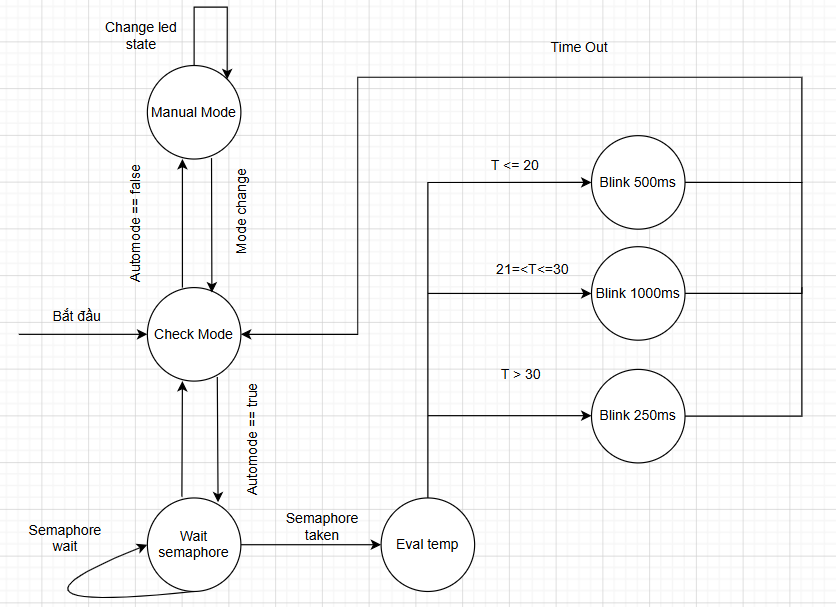
\includegraphics[width=1\linewidth]{picture/task_1_fsm.png}
 \caption{Task 1 FSM}
\end{figure}